\section{Problem Description} \label{cha:Problem_Desc}
Consider the one-dimensional boundary-value problem governing the axial deformation of a \gls{bar}. The bar has length \gls{L}
and circular cross-sectional area \glssymbol{ABar}, and \gls{z} denotes its axial coordinate. The left end is fixed, while the
axial force \gls{PBar} is applied at the right end. Let $\glssymbol{fBar}=\gls{fBar}$ denote the distributed axial load at
position $z$. We seek the displacement $\glssymbol{uBar}=\gls{uBar}$ shown in \cref{fig:Problem_Description}.

\begin{figure}
	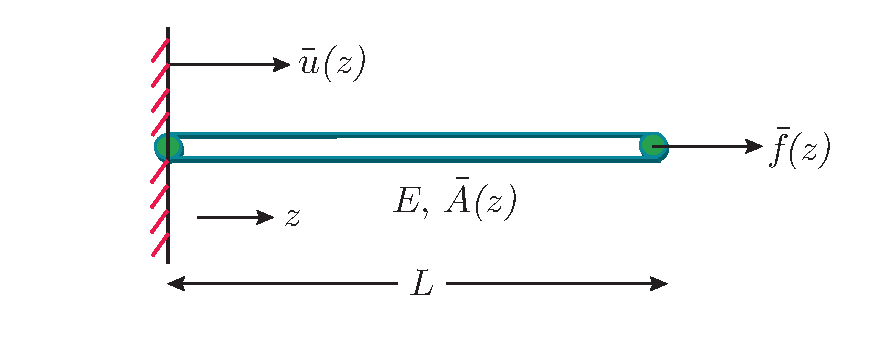
\includegraphics[width = \textwidth]{../figures/problem-description}
	\caption[A Bar Problem]
	{A One-Dimensional Bar Problem under an Axial Load}
	\label{fig:Problem_Description}
\end{figure}

